\section{Introduction}\label{sec:intro}

Landauer's principle says that resetting an unbiased bit, stored in two states of equal energy, costs at least $\kB T\ln2$ of work~\cite{Landauer61}. For $n$ uses of a quantum channel, Faist, Berta and Brand\~ao found the least work per use, the thermodynamic capacity, when the device may collect all of its inputs before it releases any output~\cite{FBB19,FBB21}: to leading order in $n$, for every channel when Gibbs-preserving maps are free, and for time-covariant channels with thermal operations. Both results describe what a device does to its inputs. Neither says when the device may touch what, and that turns out to be half of the price.

Here is the smallest case. Two bits $a$ and $b$ arrive in turn, and the device must return $a$ and then $a\oplus b$. If it may hold $a$ until $b$ arrives, one CNOT does the job and nothing is left behind. If $a$ must leave before $b$ arrives, the device must keep a copy of $a$, and once $a\oplus b$ has left too that copy is correlated only with carriers that are gone; erasing it costs $\kB T\ln2$ at any speed (Figure~\ref{fig:three}). A third schedule shows that the cost is in the release, not in the early delivery: if the device copies $a$ into a blank register, lends $a$ to the observer, and gets it back unmodified before $a\oplus b$ is due, a second CNOT uncomputes the register and the cost is again zero. The map is the same in all three cases. What changes is what the device can still reach when it has to clean up.

\begin{figure}[t]
\centering
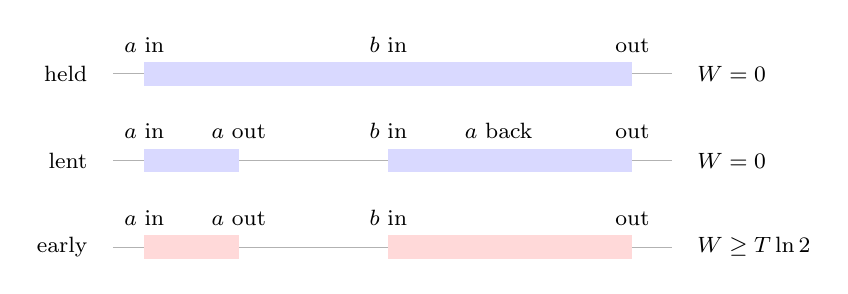
\begin{tikzpicture}[x=1cm,y=1cm,font=\footnotesize]
  \foreach \row/\y/\lab/\w in {0/2.2/held/{$W=0$}, 1/1.1/lent/{$W=0$}, 2/0/early/{$W\ge\kB T\ln 2$}} {
    \node[anchor=east] at (-0.2,\y) {\lab};
    \node[anchor=west] at (7.3,\y) {\w};
    \draw[gray!60] (0,\y) -- (7.1,\y);
  }
  % held
  \fill[blue!15] (0.4,2.05) rectangle (6.6,2.35);
  \node[above] at (0.4,2.35) {$a$ in}; \node[above] at (3.5,2.35) {$b$ in}; \node[above] at (6.6,2.35) {out};
  % lent
  \fill[blue!15] (0.4,0.95) rectangle (1.6,1.25); \fill[blue!15] (3.5,0.95) rectangle (6.6,1.25);
  \node[above] at (0.4,1.25) {$a$ in}; \node[above] at (1.6,1.25) {$a$ out}; \node[above] at (3.5,1.25) {$b$ in}; \node[above] at (4.9,1.25) {$a$ back}; \node[above] at (6.6,1.25) {out};
  % early
  \fill[red!15] (0.4,-0.15) rectangle (1.6,0.15); \fill[red!15] (3.5,-0.15) rectangle (6.6,0.15);
  \node[above] at (0.4,0.15) {$a$ in}; \node[above] at (1.6,0.15) {$a$ out}; \node[above] at (3.5,0.15) {$b$ in}; \node[above] at (6.6,0.15) {out};
\end{tikzpicture}
\caption{The same task, the same slowness, three schedules. Return $a$, then return $a\oplus b$; shaded bars show when the device can act on its carriers. Holding $a$ until $b$ arrives allows reversible cleanup, and so does lending it, provided the observer returns it unmodified before cleanup. Releasing $a$ for good strands a copy of it in the device, and the copy must be paid for. Appendix~\ref{app:classes} proves the general form: for reversible questions, the order price of a released past is the logarithm of the number of classes of pasts that later questions tell apart.}
\label{fig:three}
\end{figure}

Finite-time thermodynamics charges for speed: for protocols with a reversible quasistatic limit, the excess work due to finite speed vanishes as the protocol is slowed~\cite{SalamonBerry83,Crooks07,Proesmans20}. The charge above survives that limit. All rates in this paper allow devices of any size and any running time. Thermodynamics therefore charges for time twice: once for speed, which patience removes, and once for order, which it does not. The resource is not elapsed time. It is the capability that must remain available after access to an earlier output has been irreversibly surrendered. For classical information engines, costs that survive slow operation because processing goes step by step are known: the modularity dissipation of information ratchets~\cite{BMC18}, which Loomis and Crutchfield trace to temporal locality~\cite{LoomisCrutchfield20}, the dependence of dissipation on the input distribution a device was built for~\cite{KolchinskyWolpert17}, and the online cost of agents~\cite{Thompson25}. Those costs are forced on every implementation of a given architecture: a modular or temporally local design, a device tuned to one input distribution, an agent whose memory is a function of its past. Here the price is forced by the release schedule on every implementation, whatever its memory, and for memoryless channels it is purely quantum.

\begin{table}[tbp]
\centering
\small
\begin{tabular}{@{}>{\raggedright\arraybackslash}p{3.1cm}>{\raggedright\arraybackslash}p{10.0cm}>{\raggedright\arraybackslash}p{2.5cm}@{}}
\toprule
Result & Statement & Where\\
\midrule
One law for every schedule & For schedules whose observer-owned carriers return with their Hamiltonians, the optimal deterministic work rate is $\kB T\ln2\,K_\beta^S$, the least record entropy plus handed-over energy against the hardest observer. Lower bound: a one-page identity. Upper bound: a coherent recorder and a positive heat correction. & Theorem~\ref{to:thm:law}, Section~\ref{to:sec:law}, Appendix~\ref{app:law}\\
Only quantum channels pay for releasing & For repeated uses of one memoryless channel, each output released before the next input arrives, the real-time rate adds to the capacity's integrand, input by input, the least output--device correlation any dilation must leave, so the surcharge over the capacity is a difference of two maxima. The surcharge is zero for every classical channel; positive for partial reset at every temperature; $\kB T\ln3$ per use for Werner--Holevo, against essentially nothing in batch. Classical tasks with memory can still pay (Figure~\ref{fig:three}). & Theorems~\ref{thm:main-realtime}--\ref{thm:main-dichotomy}, Appendix~\ref{app:channels}\\
A clock has an exact price & With a returned clock, the batch cost of every channel is the single-letter quantity $B(\Phi)\ge$ capacity, with equality whenever $H-\Phi^*(H)\in\operatorname{span}\{A_i^*A_j\}$. When $H-\Phi^*(H)$ lies outside that span the channel's time orbit is Heisenberg-estimable and the clock must grow linearly; the Hadamard gate shows that $B(\Phi)$ can still equal the capacity there. & Theorem~\ref{to:thm:batchlaw}, Theorem~\ref{thm:main-heisenberg}, Appendix~\ref{app:batch}\\
What a released past must keep & Release $x$, then answer $y$ with $g(x,y)$: in real time the price is $\log_2$ of the largest fiber of $(\text{class of }x,y)\mapsto g$, when $x$ may be held it is the Landauer cost (the logarithm of the largest $y$-fiber, maximized over $x$ and the answer), and the difference, the order price, is $\log_2$ of the number of continuation classes (the causal states of the task) for reversible questions. A record is not yet a price: it can be passed into the answer. Linear tasks give a rank; deciding whether holding $m$ carriers lowers it is NP-complete. & Theorem~\ref{thm:classes}, Proposition~\ref{to:prop:rank}, Appendix~\ref{app:classes}\\
Holding is decidable, releasing is not & Batch freeness is decided by linear algebra for algebraic channel and Hamiltonian entries, when $\beta$ or the Gibbs state is algebraic. Real-time freeness of a generalized dephasing channel with cyclotomic entries is undecidable in a fixed dimension, and the free set is not recursively enumerable. & Theorem~\ref{thm:main-undecidable}, Appendix~\ref{app:channels}\\
A certificate and a protocol & A two-qubit process, free when held, costs every early-release device at least $[1-h_2(e)-e\log_23-P]\,\kB T\ln2$ per episode, where $P$ bounds the controller's and battery's budgets, which the Pauli measurements do not certify; $0.878$ at $e=1\%$ and $P=0.025$. A classical protocol with three arms, a graded control and record accounting is proposed as a design, in a feedback trap or, preferably, a preprogrammed physical memory; its record-export interface and controller bounds remain to be established. & Proposition~\ref{to:prop:certificate}, Section~\ref{sec:protocol}\\
Beyond thermodynamics & Order has a per-use price in entanglement and coherence theory as well; for the delayed-choice task one retained qubit is the common requirement, with no single exchange rate between theories. & Section~\ref{to:sec:beyond}\\
\bottomrule
\end{tabular}
\caption{Results at a glance. Entropies are in bits; $h_2$ is the binary entropy. Section~\ref{sec:contract} gives the contract and the results that depart from it.}
\label{tab:glance}
\end{table}

\paragraph{The principle.} A device is built before the observer chooses its inputs, and it must serve every observer the schedule admits. Its work rate is the least entropy that one implementation must add to its own record, plus the energy it hands over to the carriers, against the most demanding observer. Three things decide it. \emph{Access} decides which corrections remain possible: a device that still holds its outputs can erase its record using them as side information~\cite{delRio11}, as the batch construction of Faist, Berta and Brand\~ao does~\cite[Sec.~7]{FBB21}; a device that has released them cannot, and whatever its record shares with them is stranded. \emph{Universality} decides whether those corrections can belong to one device. Faist, Berta and Brand\~ao showed that in batch one device can serve every input at the cost of the hardest one~\cite{FBB19,FBB21}, and that a known i.i.d.\ input can even be served at its own free-energy cost with thermal operations and a sublinear source of coherence~\cite[Prop.~8.3]{FBB21}. With a clock that must return, one device can cost more than its hardest input (Section~\ref{to:sec:clock}). \emph{Return obligations} decide what may not be left behind as an unpaid change: a clock lent to the device must come back, and that requirement decides whether some channels can be run at all~\cite{MarvianSpekkens19,LostaglioMuller19} and, for others, what they cost.

\paragraph{Results at a glance.} Table~\ref{tab:glance} lists what the paper proves and where. Everything below is a consequence of one functional on one contract (Section~\ref{sec:contract}).

\paragraph{What the constructions are.} Every achievability statement in this paper is a statement about optimal rates. The devices that attain them are built for a number $n$ of uses known in advance, and they use clocks whose spread grows with the number of uses, startup capital that may grow without bound, and reservoirs with very large gaps; they show what is possible, not how to build an efficient or autonomous engine (Section~\ref{sec:discussion}). The lower bounds, by contrast, hold for every device at every size.

\paragraph{What is new.} The thermodynamic capacity, Landauer's bound, the side-information erasure of~\cite{delRio11}, the entropy accumulation of~\cite{DFR20} and the metrological results we invoke, the Kraus-span condition and its error-correcting code~\cite{ZhouJiang21} and their Markovian forms~\cite{ZhouZhangPreskillJiang18,DemkowiczCzajkowskiSekatski17}, are prior work, and so are the modularity and online costs of classical engines~\cite{BMC18,LoomisCrutchfield20,Thompson25} and the entanglement cost of simulating channel uses sequentially against adaptive testers~\cite{Wilde18}. Items (1)--(3) and (5) below, and the certificate of item (6), first appeared in four companion papers~\cite{Order,SaveWork,Answering,KeepingTime}, which a short letter summarizes~\cite{Letter}, and Appendix~\ref{app:companions} maps every statement taken from them. This paper consolidates those results and adds the fiber law of item (4) and the laboratory protocol of item (6). Apart from that companion work, to our knowledge the following are new.
\begin{enumerate}[label=(\arabic*),leftmargin=*,itemsep=1pt,topsep=2pt]
\item The schedule functional and the law of Theorem~\ref{to:thm:law}, with the recorder-and-dual construction that attains it for arbitrary interleavings, overlaps and loans.
\item The real-time law for channels in work units at every temperature, its strong converse at every fixed error for controllers that start thermal (a controller with a broad energy bank breaks it; whether it survives a controller whose capital has spread $o(n/\sqrt\eta)$, with $\eta$ its return error, is open; Remark~\ref{sw:rem:thermal-controller}), and the dichotomy of Theorem~\ref{thm:main-dichotomy}; at zero Hamiltonian, in units of purity, the rate and its zero set are in our earlier work~\cite{Memory,ImmediateDelivery,Douglas26closed}, with a strong converse at zero rate~\cite{Flagship}.
\item The batch law $B(\Phi)$ with a returned clock, its span criterion, and the identification of that criterion with the Hamiltonian-not-in-Kraus-span condition of Zhou and Jiang for the channel's time orbit.
\item The fiber law of Theorem~\ref{thm:classes}, which separates the order price of a released past from the Landauer cost of its answer. Its classes are the causal states of the task's $\varepsilon$-transducer~\cite{BarnettCrutchfield15}. Our tasks are in place, each answer overwriting its question, and that convention is what makes the released task of Figure~\ref{fig:three} cost $\kB T\ln2$. For classical causal agents that keep each question and write the answer to a fresh cell, Thompson et al.\ give the online cost for a given input process, which is zero for that task; their formula~\cite[Eq.~(3)]{Thompson25}, the information the memory stores about the last input and output minus what it holds about the next, is the averaged form of passing a record into an answer. New here is the worst case: neither the observers who might ask a distinguishing question nor an observer who steers the answer forces the price alone, the lower bound pairs them, and the result is the minimax price over every implementation, for devices with any memory required to serve every quantum observer with references, with an explicit small-error loss independent of the number of episodes and the private-device dimension.
\item The undecidability of real-time freeness in a fixed dimension, through the constant-sized correlation problem of Fu, Miller and Slofstra; in growing dimension, at zero Hamiltonian, it is in our earlier work~\cite{Flagship}.
\item The finite certificate of Proposition~\ref{to:prop:certificate}, and the protocol proposed in Section~\ref{sec:protocol}, built on the feedback-trap test of Landauer's principle~\cite{Jun14}. That access to a copy changes the cost of erasure is established~\cite{Bennett03,delRio11,Orlov12}, and the erasure of a fraction of a bit, the cleanup step of the graded control, has been measured in a feedback trap~\cite{Gavrilov17}. What the proposed protocol adds is a controlled release schedule with control arms, a graded helper control, and an explicit ledger of records and blank resources, whose readout interface and hardware budgets remain to be established.
\end{enumerate}

\paragraph{Reading guide.} Section~\ref{sec:contract} fixes the contract and says what it rules out. Section~\ref{to:sec:law} states the law and proves its lower bound in full. Sections~\ref{to:sec:table}--\ref{to:sec:clock} read the law on the schedules that matter most, Section~\ref{sec:classes} on tasks that release a past, and Section~\ref{to:sec:computability} on the complexity of freeness. Section~\ref{to:sec:measure} and Section~\ref{sec:protocol} are for experimenters. Section~\ref{sec:related} places the results among prior work, Section~\ref{sec:verification} says which statements are checked by machine, by formal proof and by text alone, Appendix~\ref{app:glossary} defines every term of art, and Appendix~\ref{app:companions} gives the number of every result in the companion papers. The appendices contain the proofs, complete except for two results imported from our earlier preprints, Lemma~\ref{sw:lem:smoothing} and~\cite[Thm.~3.2(a)]{Memory} (Section~\ref{sec:channel-statements}): Appendix~\ref{app:law} the law, Appendix~\ref{app:module} the physical module and the law for processes with memory, Appendix~\ref{app:channels} memoryless channels, Appendix~\ref{app:batch} the returned clock, Appendix~\ref{app:classes} continuation classes, and Appendices~\ref{to:app:release}--\ref{to:app:rank} the release lemma, the numbers of Section~\ref{to:sec:beyond}, the two-qubit certificate and release rank. A reader who wants only the mechanism can read Sections~\ref{sec:intro}--\ref{to:sec:law} and Appendix~\ref{app:classes}; a reader who wants only the experiment can read Sections~\ref{to:sec:measure}--\ref{sec:protocol}. The numbers quoted in Sections~\ref{to:sec:law}--\ref{to:sec:beyond} are recomputed, and the finite identities listed in Table~\ref{tab:verification} checked, by a deterministic verification package with negative controls (Section~\ref{sec:verification}).

\paragraph{Two layers.} The mechanism is not specific to heat; what thermodynamics adds is the form of the price and its complexity. The free energy relative to the Gibbs state splits across a release as
\begin{equation}\label{eq:split}
D(\rho_{CO}\|\gamma_C\otimes\gamma_O)=D(\rho_C\|\gamma_C)+D(\rho_O\|\gamma_O)+I(C{:}O),
\end{equation}
so at a fixed state the price of releasing $O$ from a device $C$ is a mutual information, the free energy of correlations that joint operations could have recovered~\cite{PerarnauLlobet15}. Optimized over inputs, the surcharge is a difference of two maxima rather than the largest mutual information, because the two maxima can sit at different inputs (Section~\ref{to:sec:waiting}). For classical computation this is the modularity dissipation of Boyd, Mandal and Crutchfield, the free energy of correlations lost to local control~\cite{BMC18}; here the cut is a release in time. And the set of channels that cost nothing in real time is undecidable, while its batch counterpart, and every analogue we know outside thermodynamics, is decidable.
